\documentclass[Shifrin_Solutions_Spring_2018]{subfiles}
\begin{document}


\section{The Gauss Map and the Second Fundamental Form}

\begin{exercise}
Check that if there are no umbilic points and the parameter curves are lines of curvature, then $F = m = 0$ and we have the principal curvatures $k_1 = \ell/E$ and $k_2 = n/G$. Conversely, prove that if $F =m =0$, then the parameter curves are lines of curvature.
\end{exercise}

\begin{exercise} number two

\end{exercise}

\begin{exercise} Compute the second fundamental form $\mathrm{II}_P$ of the following parametrized surfaces. Then calculate the matrix of the shape operator, and determine $H$ and $K$.
\begin{itemize}
\item[a.] the cylinder: $x(u,v) = \left( a \cos u , a \sin u , v \right) $
\item[b.] the torus: $x(u,v) = \left ( (a+b\cos u) \cos v, (a+b\cos u) \sin v , b \sin u \right) $
\item[c.] the helicoid: $x(u,v) = \left( u\cos v , u \sin v , b v \right) $
\item[d.] the catenoid: $x(u,v) = a\left( \cosh u \cos v, \cosh u\sin v, u \right) $
\item[e.] the Mercator parametrization of the sphere: $x(u,v) = \left( \sech u \cos v , \sech u \sin v, \tanh u \right) $
\end{itemize}
\end{exercise}

\begin{proof}[Solution] This is a set of direct computations. We list only the correct results.
\begin{itemize}
\item[a.] For the cylinder as given:
\begin{align*}
\mathrm{II} & = \begin{pmatrix} -a^2 & 0 \\ 0 & 0 \end{pmatrix} \\
\left[S_P\right] & = \begin{pmatrix} -1 & 0 \\ 0 & 0 \end{pmatrix} \\
H & = -1/2, \quad K = 0
\end{align*}

\item[b.] For the torus as given:
\begin{align*}
\mathrm{II} & = \begin{pmatrix} b & 0 \\ 0 & (a+b\cos u) \cos u \end{pmatrix} \\
\left[S_P\right] & = \begin{pmatrix} \dfrac{1}{b} & 0 \\ 0 & \dfrac{\cos u}{a+b\cos u} \end{pmatrix} \\
H & = \dfrac{1}{2}\left( \dfrac{1}{b} + \dfrac{\cos u}{a+b\cos u}\right), \quad K = \dfrac{\cos u}{b(a+b\cos u)}
\end{align*}

\item[c.] For the helicoid as given:
\begin{align*}
\mathrm{II} & = \begin{pmatrix} 0 & \dfrac{-b}{u^2+b^2} \\ \dfrac{-b}{u^2+b^2} & 0  \end{pmatrix} \\
\left[S_P\right] & =\dfrac{-b}{(u^2+b^2)^{3/2}} \begin{pmatrix}  0 & u^2+b^2 \\ 1 & 0 \end{pmatrix} \\
H & = 0, \quad K = \left( \dfrac{b}{u^2+b^2} \right)^2
\end{align*}

\item[d.]

\item[e.]  For the Mercator parametrization of the sphere:
\begin{align*}
\mathrm{II} & = \begin{pmatrix} \sech^2 u &  0\\ 0 & \sech^2 u \end{pmatrix} \\
\left[S_P\right] & = \begin{pmatrix} 1  & 0 \\ 0 & 1 \end{pmatrix} \\
H & = 1, \quad K = 1
\end{align*}

\end{itemize}
\end{proof}



\begin{exercise}
Find the principal curvatures, the principal directions, and asymptotic directions (when they exist) for each of the surfaces in Exercise 3. Identify the lines of curvature and asymptotic curves.
\end{exercise}

\begin{proof}[Solution]
\begin{itemize}
\item[a.] Since the shape operator is diagonal, we can read off the principal directions and curvatures: $k_1 = -1$, $e_1 = x_u$ is the $u$-direction, and $k_2 = 0$, $e_2 = x_v$ is the $v$-direction. To find asymptotic directions, use Euler's formula. $V=\cos \theta e_1 + \sin\theta e_2$ is asymptotic means that
\[
0 = \mathrm{II}(V,V) = k_1 \cos^2 \theta + k_2 \sin^2 \theta = -\cos^2 \theta.
\]
This means that $\theta$ must be equal to $\pi/2$ or $3\pi/2$. Hence, the asymptotic directions are exactly $\pm x_v$.

The lines of curvature are of two types: Those of the first type are circles. They are parallels of this surface of revolution, the $u$-curves. Those of the second type are lines. These are the profile curves of the surface of revolution, the $v$-curves, and also the rulings of this surface of revolution.

The asymptotic curves are the vertical lines traced as $v$-curves.\\


\item[b.] The shape operator is diagonal, so we see that the principal directions are the $x_u$ and $x_v$ directions. The principal curvatures are $1/b$ and $\frac{\cos u}{a+b\cos u}$. The lines of curvature are the $u$-curves, which are circles, and the $v$-curves, which are also circles. The first kind are profile curves and go around the torus the short way (through the hole), and the second kind are parallels and go around the torus the long way (around the hole).

The asymptotic directions only exist on the ``inner half'' of the torus where the second principal curvature is negative and we have hyperbolic points. In this case, we can solve the defining equation for asymptotic directions to get the following vectors
\[
\begin{pmatrix} 1 \\ \sqrt{\dfrac{-b}{(a+b\cos u) \cos u}} \end{pmatrix} = x_u + \sqrt{\dfrac{-b}{(a+b\cos u) \cos u}} x_v
\]
and
\[
\begin{pmatrix} 1 \\ -\sqrt{\dfrac{-b}{(a+b\cos u) \cos u}}\end{pmatrix} = x_u -\sqrt{\dfrac{-b}{(a+b\cos u) \cos u}} x_v .
\]

\item[c.] Solving for eigenvectors and eigenvalues of the shape operator, we find that the principal direction/curvature pairs are
\begin{align*}
e_1 &= \sqrt{u^2+b^2} x_u + x_v, \quad k_1 = \dfrac{-b}{u^2+b^2} \\
e_2 &= -\sqrt{u^2+b^2} x_u + x_v, \quad k_2 = \dfrac{b}{u^2+b^2}
\end{align*}
Finding the principal directions entails solving some ODE's, so we'll skip it.

The asymptotic directions come from solving $\mathrm{II}(V,V)=0$. Since $\mathpzc{l}$ and $\mathpzc{n}$ both vanish, it is not hard to see that the asymptotic directions are the coordinate directions. Hence asymptotic curves for the helicoid are the $u$-curves and $v$-curves. The $v$-curves are helices, and the $u$-curves are rulings.


\item[d.]

\item[e.] The shape operator is the identity matrix. Hence every direction is a principal direction and all the principal curvatures are equal to $+1$. But since all are equal, none are special\dots so it really is better to pretend there are not principal directions here. All points are umbilics. There are no asymptotic curves, and in a sense any curve should be a line of curvature, but again, it seems better to say that no curve is.

\end{itemize}
\end{proof}

%%%%%%%%%%%%%%%%%%%%%%%%%%%%%%%%%%%%%%%%%%%%%%%%%%%%%%%%%%%%%%%%%%%%%%%%%%%%%%%%%%%555
\begin{exercise}
Prove by calculation that any one of the helices $\alpha(t) = \left( a\cos t , a\sin t , bt\right)$ is an asymptotic curve on the helicoid given in Example 1(b) of section 1. Also, calculate how the surface normal $n$ changes as one moves along the ruling, and use this to explain why the rulings are asymptotic curves as well.
\end{exercise}

\begin{proof}[Solution]
It is pretty clear from our work in the last problem that these helices are asymptotic. For a change, let's compute a totally different way. Recall that $\mathrm{II}(V,V) = \left( -D_{V}n\right) \cdot V$ by definition. We shall use this with $V = \alpha'$. Also, the derivative that must be taken is along the curve, so really $D_{\alpha'}n = (n\circ \alpha)'(t)$. With this in mind, we can compute as follows:
\begin{align*}
n\circ \alpha(t) = \dfrac{1}{\sqrt{a^2+b^2}} \left( b \sin t , -b \cos v , a \right) \\
(n\circ \alpha)'(t) = \dfrac{1}{\sqrt{a^2+b^2}}\left( b\cos t , b \sin t , 0 \right)\\
\alpha'(t) = \left( -a\sin t , a\cos t , b\right) \\
\mathrm{II}_{\alpha(t)}(\alpha'(t), \alpha'(t) ) = (n\circ\alpha)'(t) \cdot \alpha'(t) = 0.
\end{align*}

Now, along a ruling (that is, a $u$-curve), the normal looks like this
\[
n(u,v_0) = \left( \dfrac{b\sin v_0}{\sqrt{u^2 + b^2}} , \dfrac{b\sin v_0}{\sqrt{u^2 + b^2}} , \dfrac{u}{\sqrt{u^2 + b^2}}\right).
\]
So, if we take a derivative in the $u$-direction, we see
\[
\begin{split}
n_u (u,v_0) & = \left( \dfrac{-ub\sin v_0}{(u^2+b^2)^{3/2}}, \dfrac{ub\cos v_0}{(u^2+b^2)^{3/2}} , \dfrac{b^2}{(u^2+b^2)^{3/2}}\right) . \\
	& = \dfrac{b}{(u^2+b^2)^{3/2}} x_v
\end{split}
\]
Since we have seen that $F = x_u\cdot x_v = 0$, we deduce that the derivative of $n$ along the rulings is orthogonal to the rulings. This means that $\mathrm{II}(x_u,x_u) = -D_{x_u} \cdot x_u =0$, that is, the rulings are asymptotic curves.
\end{proof}

%%%%%%%%%%%%%%%%%%%%%%%%%%%%%%%%%%%%%%%%%%%%%%%%%%%%%%%%%%%%%%%%%%%%%%%%%%%%%%%%%%%%%%%%5
\begin{exercise}
number six
\end{exercise}

%%%%%%%%%%%%%%%%%%%%%%%%%%%%%%%%%%%%%%%%%%%%%%%%%%%%%%%%%%%%%%%%%%%%%%%%%%%%%%%%%%%%%%%%
\begin{exercise}
Show that a ruled surface has Gaussian curvature $K\leq 0$.
\end{exercise}

\begin{proof}[Solution]
This proof is computational, and we highlight only the crucial parts of the computation. Write the ruled surface as $x(u,v) = \alpha(u)+ v\beta(u)$. Then $x_v = \beta$ and $x_{vv} = 0$. Hence $\mathpzc{n} = n\cdot x_{vv} = 0$. Now we see that
\[
K = \dfrac{\mathpzc{l}\mathpzc{n}- \mathpzc{m}^2}{EG-F^2} = - \dfrac{ \mathpzc{m}^2}{EG-F^2} \leq 0 .
\]
\end{proof}

%%%%%%%%%%%%%%%%%%%%%%%%%%%%%%%%%%%%%%%%%%%%%%%%%%%%%%%%%%%%%%%%%%%%%%%%%%%%%%%%%%%%%%%%%%
\begin{exercise}
\begin{itemize}
\item[a.] Prove that the principal directions bisect the asymptotic directions.
\item[b.] Prove that if the asymptotic directions of $M$ are orthogonal, then  $M$ is minimal. Prove the converse assuming $M$ has no planar points.
\end{itemize}
\end{exercise}

\begin{proof}[Solution]
By Euler's formula, if $V^{\ast}= V(\theta^\ast) = \cos \theta^{\ast} e_1 + \sin \theta^{\ast} e_2$ is asymptotic, then
\[
0 = \mathrm{II}(V^\ast, V^\ast) = k_1\cos^2\theta^\ast + k_2 \sin^2\theta^\ast .
\]
This means that $-k_1/k_2 = \tan^2 \theta^\ast$. In order to have asymptotic directions, we may assume that $k_1 \leq 0 < k_2$, so it makes sense to find $\theta^\ast$ by solving this equation. It helps to look at the graphs of $\tan^2$ and a horizontal line.

\begin{figure}[h]
\centering
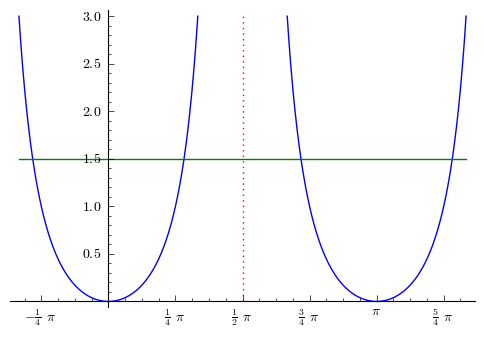
\includegraphics[width=.5\textwidth]{picturebook/ch2sec2/tan2-graph}
\caption{The graph of $y= \tan^2 x$ and a typical horizontal line.}
\end{figure}

From the figure, we can recall that the solutions to $\tan^2\theta = C$ satisfy some symmetry relations. If $\theta$ is a solution, so are $\theta+ \pi$ and $-\theta$. Putting these together, we see that $\pi - \theta$ is also a solution.

\begin{itemize}
\item[a.] It is now clear that $e_1$ bisects the asymptotic directions $V(\theta^\ast)$ and $V(-\theta^\ast)$, and $e_2$ bisects the asymptotic directions $V(\theta^\ast)$ and $V(\pi - \theta^\ast)$.

\item[b.] Suppose that the asymptotic directions are orthogonal. If $V(\theta^\ast)$ and $V(\psi^\ast)$ are asymptotic directions (with consecutive values of the angle), then $\tan^2\theta^\ast = \tan^2\psi^\ast$. Since they are orthogonal, their angles differ by $\pi/2$. Without loss of generality, assume that $\theta^\ast = \psi^\ast + \pi/2$, and $\psi^\ast < 0 < \theta^\ast$. By the symmetries of $tan^2$, we see that $\psi^\ast = - \theta^\ast$. This means that the angles must be $\pm \pi/4$. Using the work above, we new see that $-k_1/k_2 = \tan^2\theta^\ast = 1$. This means that the principal curvatures have the same modulus but opposite signs, so $H=0$. Thus $M$ is minimal.

Now suppose that $M$ is minimal. Then $-k_1=k_2$, so by Euler's formula the normal curvature in the asymptotic direction $\theta$ is
\[
\begin{split}
0 & = k_1 \cos^2\theta + k_2 \sin^2\theta \\
	& = k_1 \left( cos^2\theta - \sin^2\theta \right) \\
	& = k_1 \cos(2\theta)
\end{split}
\]
If there are no planar points, we know $k_1 \neq 0$, so $\cos(2\theta) = 0$. This equation has solutions of the form $\pi/4 + \pi k$ and $3\pi/4 + \pi k$ where $k$ is allowed to be any integer. We now see that the asymptotic directions are orthogonal.
\end{itemize}
\end{proof}

%%%%%%%%%%%%%%%%%%%%%%%%%%%%%%%%%%%%%%%%%%%%%%%%%%%%%%%%%%%%%%%%%%%%%%%%%%%%%%%%%%%%%%%%%%555
\begin{exercise}
number nine, number nine, number nine\dots
\end{exercise}

%%%%%%%%%%%%%%%%%%%%%%%%%%%%%%%%%%%%%%%%%%%%%%%%%%%%%%%%%%%%%%%%%%%%%%%%%%%%%%%%%%555
\begin{exercise}
Consider the ruled surface $M$ given by $x(u,v) = \left( v\cos u, v\sin u , uv \right)$, $v>0$.
\begin{itemize}
\item[a.] Describe this surface geometrically.
\item[b.] Find the first and second fundamental forms and the Gaussian curvature of $M$.
\item[c.] Check that the $v$-curves are lines of curvature.
\item[d.] Proceeding somewhat as in Example 6, show that the other lines of curvature are given by the equation $v\sqrt{1+u^2}= c$ for various constants $c$. Show that these curves are the intersections of $M$ with the spheres $x^2+y^2+z^2 = c^2$.
\end{itemize}
\end{exercise}

\begin{proof}[Solution]
\begin{itemize}
\item[a.] This surface is a cone made of rays from the origin through the points of the helix $(\cos u, \sin u, u)$.

\item[b.] This part is computational, and the correct results are
\begin{align*}
\mathrm{I} & = \begin{pmatrix} 2v^2 & uv \\ uv & 1+u^2 \end{pmatrix} \\
\mathrm{II} & = \begin{pmatrix} -\dfrac{uv}{\sqrt{2+u^2}} & 0 \\ 0 & 0 \end{pmatrix} \\
K = \dfrac{\det(\mathrm{II})}{\det(\mathrm{I})} = 0
\end{align*}

\item[c.] If we compute the coordinate representation of the shape operator, we obtain
\[
\left[ S_P\right] = \mathrm{I}^{-1} \mathrm{II} = \dots = \dfrac{-u}{v(u^2+2)^{3/2}} \begin{pmatrix} 1+u^2 & 0 \\ -uv & 0 \end{pmatrix} .
\]
From this it is clear that the $v$ direction is an eigendirection for eigenvalue $0$. Thus the $v$-curves are lines of curvature.


\item[d.] To find the other lines of curvature, we need to find the other eigenvector for the shape operator. If we write $A = a_1 x_u + a_2 x_v \equiv \begin{smallmatrix} a_1 \\ a_2 \end{smallmatrix}$ for this eigenvector with corresponding eigenvalue $\lambda$ we see
\[
\begin{split}
\begin{pmatrix}0\\0\end{pmatrix} & = \left[ S_P\right] A -\lambda A \\
	& = \begin{pmatrix} \left(\dfrac{-u(1+u^2)}{v(u^2+2)^{3/2}}- \lambda \right)a_1 \\ \left(\dfrac{u^2}{(u^2+2)^{3/2}} a_1 - \lambda a_2\right) \end{pmatrix}
\end{split}
\]
The first coordinate equation tells us that $\lambda = \dfrac{-u(1+u^2)}{v(u^2+2)^{3/2}}$, and then the second equation tells us (after clearing common factors) that $uv a_1 + (1_u^2)a_2 = 0$. Hence our eigenvector is
\[
A = \begin{pmatrix} 1+u^2 \\ -uv \end{pmatrix} \equiv (1+u^2)x_u - uv x_v .
\]
Now, we wish to find the lines of curvature. It is easier to work in the parameter space than in $\mathbb{R}^3$. So, the corresponding curves in the $uv$-plane have direction $(u', v') = (1+u^2, -uv)$. We thus obtain the differential equation
\[
\dfrac{dv}{du} = \dfrac{dv/dt}{du/dt} = \dfrac{v'}{u'} = \dfrac{-uv}{1+u^2} .
\]
Separating variables and integrating, we obtain $\ln v = -1/2 \ln (1+u^2) + C$, where $C$ is some constant of integration. This equation is equivalent to $v\sqrt{1+u^2} = c$, where $c=e^C$ is a different constant, but still a constant.

It is now a simple matter to check that the curves $\alpha_c(u) = x\left(u, \dfrac{c}{\sqrt{1+u^2}}\right)$ lie on the spheres $x^2+y^2+z^2=c^2$, and also that such a sphere intersects our surface at a set of points which satisfy $v^2(1+u^2)  = c^2$. Therefore, the lines of curvature we are after are exactly the intersection of our surface with the spheres centered at the origin. It is nice to draw a picture of this situation, and we get a very pretty picture where the lines of curvature we just found show up as pretty spherical spirals.

\begin{figure}[hb]
\centering
\subfloat[The Cone on a Helix]{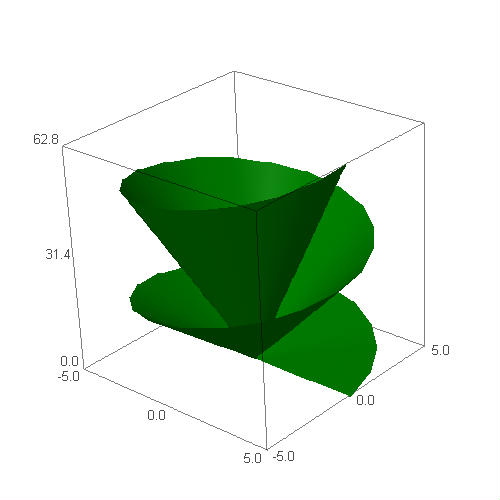
\includegraphics[width=.48\textwidth]{picturebook/ch2sec2/cone-on-helix}}
\subfloat[The Lines of Curvature]{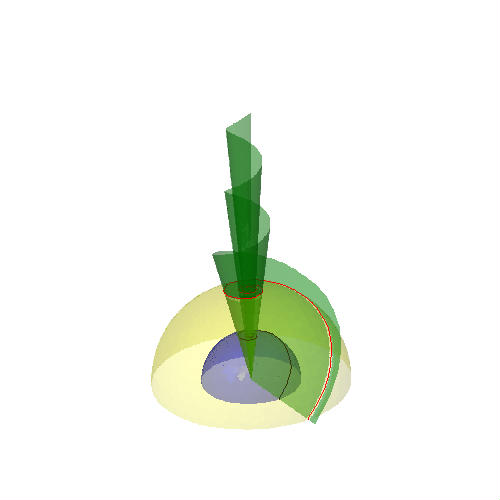
\includegraphics[width=.48\textwidth]{picturebook/ch2sec2/cone-on-helix-lines-curvature}}
\caption{The Surface of Problem 10}
\end{figure}
\end{itemize}
\end{proof}


%%%%%%%%%%%%%%%%%%%%%%%%%%%%%%%%%%%%%%%%%%%%%%%%%%%%%%%%%%%%%%%%%%%%%%%%%%%%%%%%%%%
\begin{exercise}
The curve $\alpha(t) = x(u(t), v(t))$ may arise by writing $\dfrac{dv}{du} = \dfrac{v'(t)}{u'(t)}$ and solving a differential equation to relate $u$ and $v$ either explicitly or implicitly.
\begin{itemize}
\item[a.] Show that $\alpha$ is an asymptotic curve if and only if $\mathpzc{l}(u')^2 + 2\mathpzc{m}u' v' + \mathpzc{n}(v')^2 = 0$. Thus if $\mathpzc{l} + 2\mathpzc{m}\dfrac{dv}{du} + \mathpzc{n}\left(\dfrac{dv}{du}\right)^2 = 0$, then $\alpha$ is an asymptotic curve.

\item[b.] Show that $\alpha$ is a line of curvature if and only if $\begin{vmatrix}
Eu' + Fv' & Fu'+Gv' \\ \mathpzc{l}u' + \mathpzc{m}v' & \mathpzc{m}u' + \mathpzc{n}v'
\end{vmatrix} =0$. Give the appropriate condition in terms of $dv/du$.

\item[c.] Deduce that an alternate condition for $\alpha$ to be a line of curvature is that
\[
\begin{vmatrix}
(v')^2 & -u'v' & (u')^2 \\
E & F & G \\
\mathpzc{l} & \mathpzc{m}  & \mathpzc{n}
\end{vmatrix}
=0.
\]
\end{itemize}
\end{exercise}

\begin{proof}[Solution]
That the curve $\alpha$ is asymptotic means that its tangent vector $\alpha' = u' x_u + v' x_v$ is always an asymptotic vector. That is
\[
0 = \mathrm{II}(\alpha' , \alpha') = \mathpzc{l}(u')^2 + 2\mathpzc{m}u'v' + \mathpzc{n}(v')^2 .
\]
The condition in part (a.) comes from dividing through by $(u')^2$ and recalling that $dv/du = v'/u'$.\\

To be a line of curvature, means that $\alpha' = u'x_u + v'x_v$ is always an eigenvector of  the shape operator. In coordinate form this means that if we view the first and second fundamental forms as matrices, then
\[
\mathrm{I}^{-1}\mathrm{II}(\alpha') = \lambda \alpha' .
\]
This is the same thing as the condition that $\mathrm{II}(\alpha') = \lambda \mathrm{I}(\alpha')$, or that $\mathrm{I}(\alpha')$ and $\mathrm{II}(\alpha')$ are linearly dependent. Since
\begin{align*}
\mathrm{I}(\alpha') & =\begin{pmatrix} Eu' + Fv' \\ F u' + Gv' \end{pmatrix}, \text{ and} \\
\mathrm{II}(\alpha') &  = \begin{pmatrix}\mathpzc{l} u' + \mathpzc{m}v' \\ \mathpzc{m}u' + \mathpzc{n}v' \end{pmatrix} ,
\end{align*}
this is clearly the same as the determinant condition given in part (b.). To restate it in terms of a differential equation, we divide through the top and bottom rows of the determinant by $u'$, replace $v'/u'$ by $dv/du$, and evaluate the determinant to find the differential equation
\[
\left(E\mathpzc{m} - \mathpzc{l}F\right) + \left( E\mathpzc{n} - \mathpzc{l}G\right) \dfrac{dv}{du} + \left( F\mathpzc{n} - \mathpzc{m}G\right) \left( \dfrac{dv}{du}\right)^2 = 0.
\]
Of course, if we hadn't cleared the $u'$'s we would have found this equation
\[
\left(E\mathpzc{m} - \mathpzc{l}F\right)(u')^2 + \left( E\mathpzc{n} - \mathpzc{l}G\right) u'v' + \left( F\mathpzc{n} - \mathpzc{m}G\right) (v')^2 = 0.
\]
This last equation is clearly the same as the $3\times 3$ determinant identity in part (c.).


\end{proof}

%%%%%%%%%%%%%%%%%%%%%%%%%%%%%%%%%%%%%%%%%%%%%%%%%%%%%%%%%%%%%%%%%%%%%%%%%%%%%%%%%%%%555
\begin{exercise}
number twelve
\end{exercise}

%%%%%%%%%%%%%%%%%%%%%%%%%%%%%%%%%%%%%%%%%%%%%%%%%%%%%%%%%%%%%%%%%%%%%%%%%%%%%%%%%%%%%%%%5
\begin{exercise}
lucky thirteen
\end{exercise}

%%%%%%%%%%%%%%%%%%%%%%%%%%%%%%%%%%%%%%%%%%%%%%%%%%%%%%%%%%%%%%%%%%%%%%%%%%%%%%%%%%%555
\begin{exercise}
Suppose that for every $P \in M$, the shape operator $S_P$ is some scalar multiple of the identity, i.e. $S_P(V) = k(P)V$ for all $V \in T_PM$. (Here the scalar $k(P)$ may well depend on the point $P$.)
\begin{itemize}
\item[a.] Differentiate the equations
\begin{align*}
D_{x_u} n & = n_u  = -k x_u \\
D_{x_v} n & = n_v  = -k x_v
\end{align*}
appropriately to determine $k_u$ and $k_v$ and deduce that $k$ must be a constant.

\item[b.] We showed in Proposition 2.2 that $M$ is planar when $k=0$. Show that when $k\neq 0$, $M$ is (a portion of) a sphere.
\end{itemize}
\end{exercise}

\begin{proof}[Solution]
We begin by differentiating in a way to obtain mixed parital derivatives of the normal $n$.
\begin{align*}
n_{uv} = -k_v x_u - k x_{uv}, \\
n_{vu} = -k_u x_v - k x_{vu} .
\end{align*}
Since mixed paritals are equal, we see that the left-hand sides are equal and the last terms on the right-hand side are equal. Hence $k_v x_u = k_u x_v$. However, for a regular surface $x_u$ and $x_v$ are linearly independent, so $k_u=k_v=0$. This means that $k$ is a constant.\\

Now, if $k\neq 0$ but is constant, we wish to show that $M$ is a portion of a sphere. Consider the vector $P = x + \dfrac{1}{k} n$.  Because $k$ is a constant,
\[
\dfrac{d}{du} ||P||^2 =2 \left( x + \dfrac{1}{k}n\right) \cdot \left( x_u + \dfrac{1}{k} n_u\right) = 2\left( x + \dfrac{1}{k}n\right) \cdot \left( x_u + \dfrac{1}{k}(-k x_u)\right) = 0,
\]
and similarly for the $v$ derivative. Therefore, $P$ is a constant. This is the center of our sphere. Since the norm of $n$ is always $1$, the above proves that $x$ lies on the sphere centered at $P$ with radius $1/k$.
\end{proof}

%%%%%%%%%%%%%%%%%%%%%%%%%%%%%%%%%%%%%%%%%%%%%%%%%%%%%%%%%%%%%%%%%%%%%%%%%%%%%%%%%%%%%%%%%%%%5
\begin{exercise}

\end{exercise}


\begin{exercise}

\end{exercise}


\begin{exercise}

\end{exercise}


\begin{exercise}

\end{exercise}


\begin{exercise}

\end{exercise}


\begin{exercise}

\end{exercise}

\begin{exercise}

\end{exercise}


\begin{exercise}

\end{exercise}


\begin{exercise}

\end{exercise}


\begin{exercise}

\end{exercise}

\end{document}
